%% -*- mode: latex; mode: reftex; mode: flyspell; TeX-master: "top.tex"; -*-
\vspace{-3mm}
%----------------------------------------------------------------------------
\begin{figure*}[t!]
  \centering
       \begin{tabular}{@{}c@{\hspace{2mm}}c@{\hspace{2mm}}c@{}}
         {\footnotesize (a) Maximum Distance from Neurite Tip to Soma} &
         {\footnotesize (b) $\Delta$ Neurite Elongation} &
	 {\footnotesize (c) Nucleus Speed}\\
%	 {\footnotesize (d) Maximum Number of Branches in Neurite} \\ %[-1ex]
        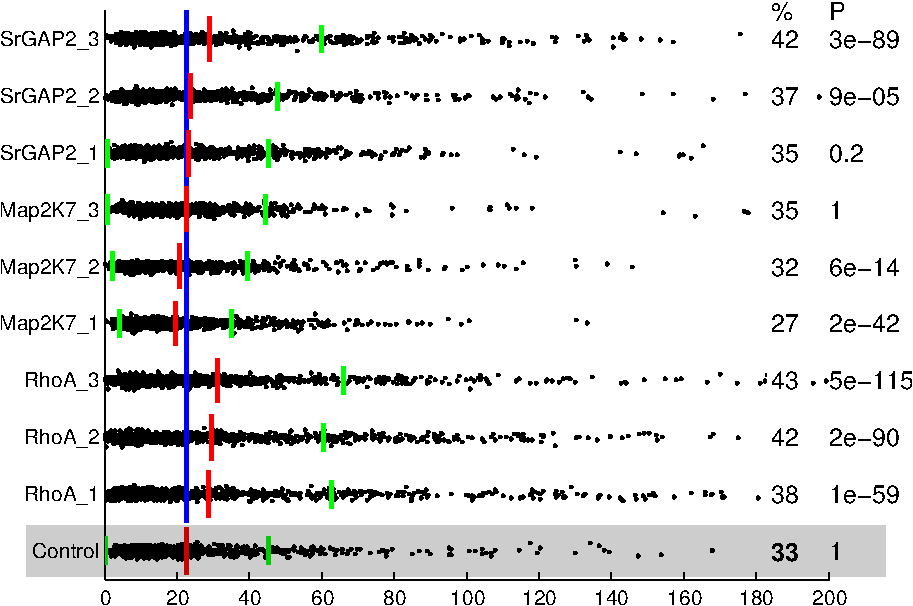
\includegraphics[height = 38mm] {images/DistToSomaExtremeNeurite.pdf} &
        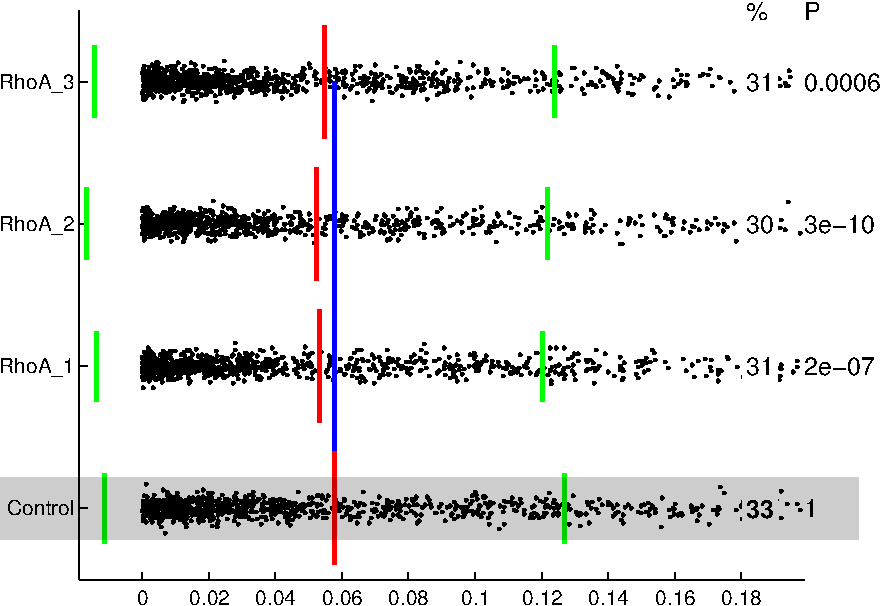
\includegraphics[height = 38mm] {images/EccentricityNeuriteDelta.pdf} &
        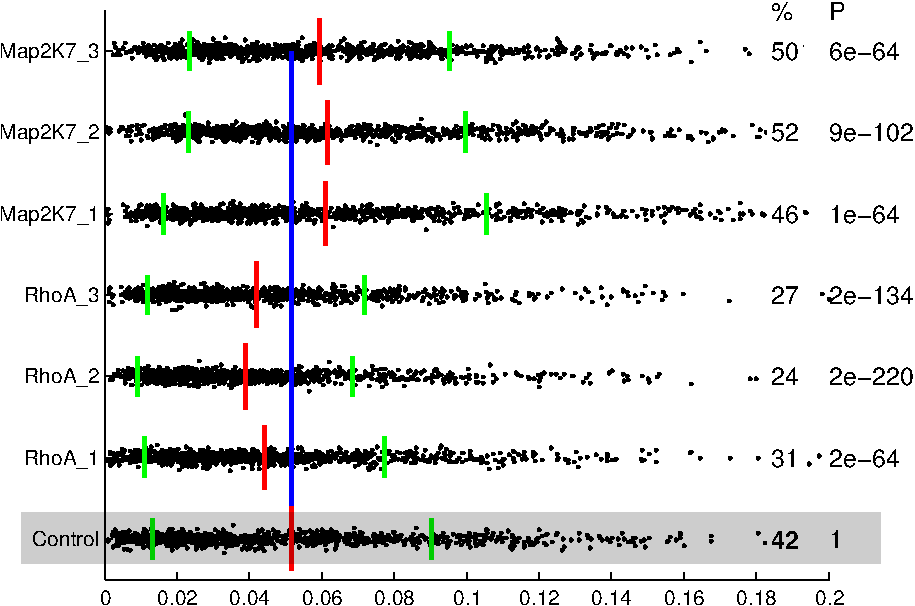
\includegraphics[height = 38mm] {images/SpeedNuclei.pdf} \\ [-1ex]
%        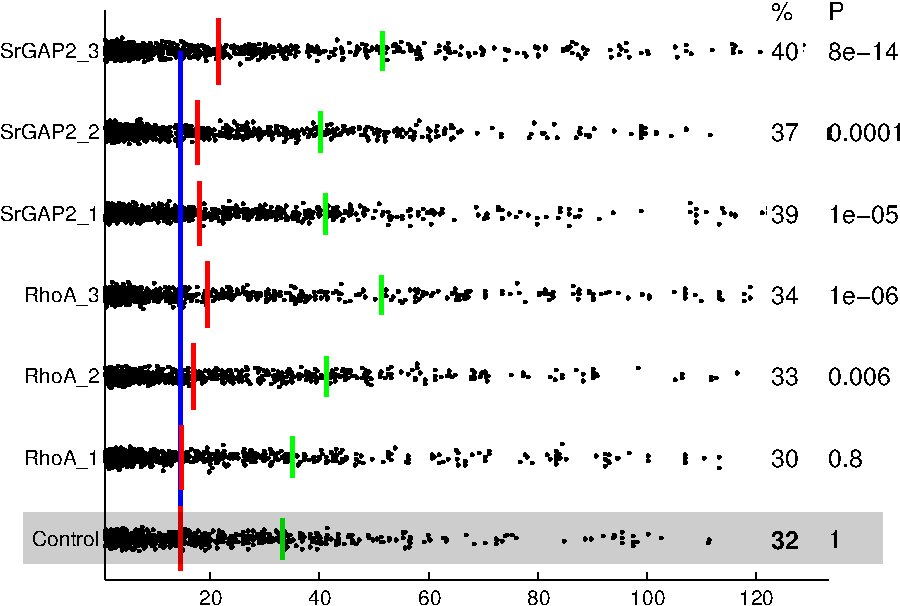
\includegraphics[height = 38mm] {images/MaxBranchCountNeurite.pdf} \\ [-1ex]
	{\footnotesize $\mu$m} & Elongation &        
%        {\footnotesize $\mu$m/min } & {\footnotesize Number of branches} \\ [-2.2ex]
	{\footnotesize $\mu$m/min } \\ [-2.2ex]
       \end{tabular} 
    \caption{ \footnotesize Morphodynamic analysis of 3/156 informative features
      out system extracts.  The control is marked in  gray.  Black dots indicate
      collected data  points.  Red bars  indicate the mean, green  bars indicate
      standard deviation.   The control  mean is shown  by a blue  line.  Values
      under the $\%$ column show the percentage of data points below the control
      mean.  The  P column  reports the statisical  signifcance measured  by the
      student-t test  $p$-value.  {\em (a)}  Our analysis confirmed  the finding
      from~\cite{Pertz08} that RhoA and  SrGAP2 loss results in longer neurites,
      and Map2K7 loss  results in shorter neurites. {\em (b)}  The low change in
      neurite elongation associated with loss of RhoA quantifies the observation
      that RhoA  loss limits the cell's  ability to retract  neurites. {\em (c)}
      Our  analysis   revealed  that  loss  of   Map2K7  and  RhoA   led  to  an
      enhancement/retardation of nucleus speed,  which was impossible to observe
      through static analysis.  }
    \label{fig:quantitative_analysis}
    %\vspace{-7mm}
\end{figure*}
%----------------------------------------------------------------------------

%% \subsection{Experimental Setup}
We applied our approach to data from a small-scale siRNA screen in which 
the functions of 5 genes were inhibited: SrGAP2, MAP2K7, RhoA, Trio, and 
Net. Three siRNAs were applied for each gene, producing a total  of 17  
experiments  including  2  controls. 30  videos  per
experiment were obtained over the  course of 3 days, with images taken
at 20$\times$ magnification 
in  10 minute intervals.  A  total of  510 videos were collected,  each containing
approximately 100 2-channel images  of $696 \times 520$ resolution.
We tracked and segmented a total of 7,298 neurons (33,213 neurites), 
extracting morphodynamic features for each. A video took under 210 seconds 
to process on a notebook computer. The entire screen was
processed in just a few hours using conventional PCs.








\subsection{Analysis}
Our goals were to 1) validate our approach by reproducing the findings 
of~\cite{Pertz08}, 2) quantify previously observed but unmeasured morphodynamics,
and 3) uncover  new dynamic behaviors.
A brief summary of our findings is provided below and in 
Fig~\ref{fig:quantitative_analysis}. Further details can be found in our 
supplementary tables and videos.
%\href{http://www.kev-smith.com/ISBI2013/}{online supplementary tables and videos}.
The findings reported below all have statistically  significant measures,  with 
a $p$-value $<< 0.05$.


Our analysis confirmed several effects previously observed through static image
analysis  in~\cite{Pertz08}.  In  particular,  RhoA  loss  of  function
resulted in fewer but longer neurites than the control. SrGap loss was
found to have longer neurites, and  Map2K7 loss was found to have
more neurites but of shorter length.  These findings  were confirmed by 
static measures from
our experiments: the mean longest  neurite length -- control $22.6 \mu
m$, RhoA-3 $32  \mu$m, SrGap2-1 $28.9 \mu$m,  and Map2K7-1 $19.5 \mu$m  
(see  Fig.~\ref{fig:quantitative_analysis}a);  and  by  a  dynamic
measure --  the mean  number of neurites  belonging a neuron  over its
lifetime: control 3.4, RhoA 3.1, and Map2K7-1 3.9.

It  had been previously observed, but  never quantified,  that  loss of
SrGap2 function  produces a  high number of  filopodia, and  that RhoA
loss  results  in neurites  that  easily  extend  but have  difficulty
retracting. Morphodynamic features from our analysis confirmed these
observations. Mean number of filopodia detected per  neurite over its lifetime was $6.69$
in the control  and $8.81$ for SrGap-3$^1$. The  mean change in elongation
as measured  by an ellipse fitted  to the neurite was  $5.7\%$ for the
control        and        $5.3\%$        for        RhoA-1        (see
Fig.~\ref{fig:quantitative_analysis}b)$^1$. While this difference may seem
small,  it is  statiscially significant due  to the  large amount  of  data collected
($p$-value is $2 \times 10^{-7}$).

Our quantitative analysis revealed new morphodynamics which
were not obvious to human  observers. We found that RhoA function loss
slowed  neuron motility and  Map2K7 increased  it.  Control cells
moved at  .30 $\mu  m / min$,  RhoA moved  at .23 $\mu  m /  min$, and
Map2K7-2     moved     at    .37     $\mu     m     /    min$     (see
Fig.~\ref{fig:quantitative_analysis}c).  We  also found that  RhoA and
SrGap  increased the  branching of  the
neurites.
%(see Fig.~\ref{fig:quantitative_analysis}d).  
Over the course
of a  neurites lifetime, the maximum  number of branches  in a control
neuron    was    14.5,   19.44    for    RhoA-3,    and   21.39    for
SrGap2-3\footnote{Only neurons containing  the  $10^{th}$  percentile  of
  longest neurites were considered.}.





%%----------------------------------------------------------------------------
%\begin{figure}[t!]
%  \centering
%       \begin{tabular}{@{\hspace{-2mm}}c@{\hspace{1mm}}c@{}}
%         {\tiny (a) Maximum Distance from Neurite Tip to Soma} &
%         {\tiny (b) $\Delta$ Eccentricity of an Ellipse Fitted to Neurite} \\
%        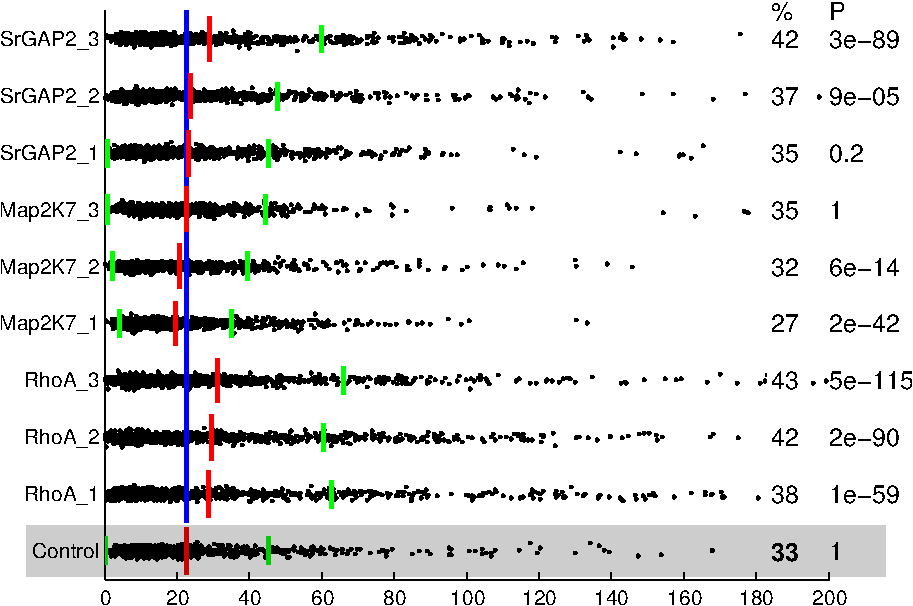
\includegraphics[height = 28mm] {images/DistToSomaExtremeNeurite.pdf} &
%        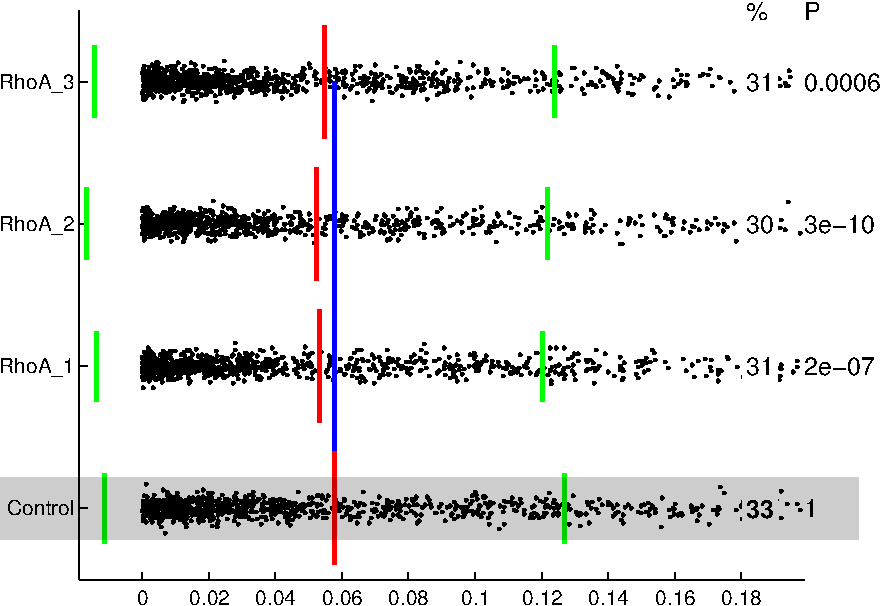
\includegraphics[height = 28mm] {images/EccentricityNeuriteDelta.pdf} \\ [-1ex]
%        {\tiny $\mu m$} & \\
%        {\tiny (c) Nucleus Speed} &
%        {\tiny (d) Maximum Number of Branches in Neurite} \\ [-1ex]
%        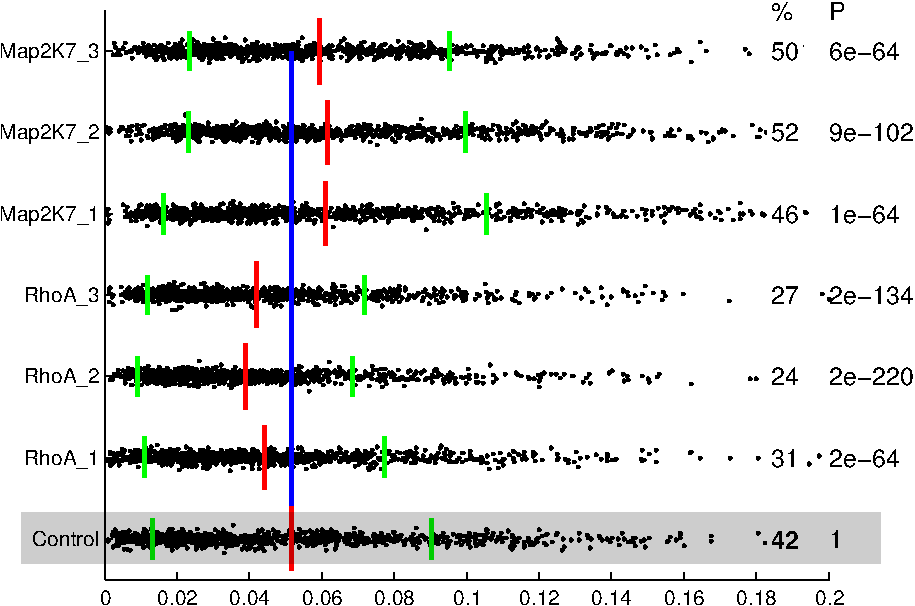
\includegraphics[height = 28mm] {images/SpeedNuclei.pdf} &
%        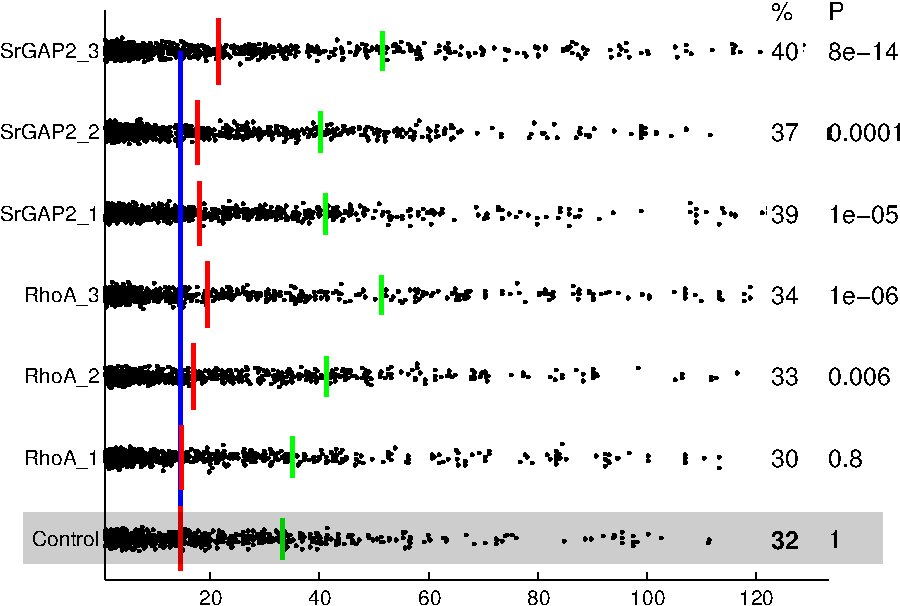
\includegraphics[height = 28mm] {images/MaxBranchCountNeurite.pdf} \\ [-1ex]
%        {\tiny $\mu m$/min } & \\ [-2.2ex]
%       \end{tabular} 
%    \caption{    {\footnotesize   {\it    Quantitative   Morphodynamic
%          Analysis.}  Four   informative  morphodynamic  features  are
%        plotted, where the control  experiment is marked in gray below
%        the  siRNA  targets.   Black  dots  represent  collected  data
%        points.  Red  bars  indicate  the mean,  green  bars  indicate
%        standard deviation.  The blue line shows the  control's mean for
%        comparison. Values under the $\%$ column are the percentage of
%        data  points  above  the  control's  mean.  Values  under  $P$
%        indicate the student-t test $p$-value. See text for details.}}
%    \label{fig:quantitative_analysis}
%    %\vspace{-7mm}
%\end{figure}
%%----------------------------------------------------------------------------






%Our analysis investigated  the effects  of  inhibiting
%various gene  functions on each  of the 156 extracted morphodynamic  features.



%Our  quantitative  analysis  investigated  the effects  of  inhibiting
%various gene  functions on each  of the 156 morphodynamic  features we
%extracted     from    our     segmentations     as    described     in
%Sec.~\ref{sec:features}.   We  summarize  our  findings below  and  in
%Fig~\ref{fig:quantitative_analysis}. We also  provide a detailed table
%and  video  results in  the  supplementary  material.  Throughout  the
%pipeline, many potential sources of noise exist, including variability
%in   neuron   behavior,   transfection   effects,  mistakes   in   our
%segmentation, and  imaging conditions.  The sheer number  of cells and
%neurites  analyzed  helps  to  average  out the  noise.  Our  findings
%reported  below are statistically  significant, all  having $p$-values
%$<< 0.05$.

%% Our approach
%% is designed to be efficient for analyzing high-throughput 
%% datasets.
%% a series of algorithm that
%% we presented

%% whole system
%% efficient

%% system is validated thorugh corroboration previous findings
%% confirmed anectocla findings
%% uncovered new dynamic phenotypes

%% biological context out of scope, future work will concentrate on that
%and addressing failure modes

%Our could be applied many other screens do more serious investiagation.


%% max branching points over  neurite lifetime
%% control  14.55
%% RhoA-3  19.44
%% SrGap2-3  21.39

%% speed
%% control   $ 9.91  \mu m / s $
%% RhoA-2    7.45
%% SrGap2-2    11.78
%% Map2K7-2   0.37
%%  0.3097    0.2328    0.3681


% eccentricity per neurite per time frame
% control 0.82
% RhoA-2 0.843  p-value  $4 \times 10^{-74}$

%% delta eccentricity
%% RhoA-1 $5.3\%$ change  $p-value$ $2 \times 10^{-7}$
%% Control $5.7\%$ change


%% over lifetime
%% RhoA_1 3.1 
%% Control 3.4
%% SrGap2_1 4.1  
%% Map2K7_1 3.9

%% 6.7 filo/neurite control



%supplementary material

%% say  how high throughput  gets rid  of noise,  and makes  our findings
%% statistically significant. talk about many sources of noise


%% p-value





%% note: make sure to say that we do not track everything - only reliably stained cells.

%% how long does it take to process?
%% It takes approximately 2.26 seconds to process each frame on a Lenovo W510 notebook computer.

%% image 97 frames 10 minute interval, 16 to 18 hours

%% In  total,  we   analyzed  $420$  video  sequences.







%\subsection{Experimental Methodology}

%\subsection{Biological Conclusions}
